\documentclass[border=4pt,12pt]{standalone}
% House style for redrawn exam diagrams (diagram-v4: 0.4pt lines, filled -latex arrows, fine dashes; stipple and hatching drawn as real dots/lines (no PDF/SVG patterns, so they render in every browser and at any scale); transparent background). Every figure \input's this.
\usepackage{amsmath,amssymb}
\usepackage{txfonts}
\usepackage{pdfrender,xcolor}
% \halo{text}: label on shading. The shading stops just around each letter's outline (a thin knock-out that follows the
% glyphs, like the papers' typesetting), never a box. Owner: "I don't want a box around the text".
\newcommand{\halo}[1]{\leavevmode\rlap{\pdfrender{TextRenderingMode=2,LineWidth=2.2pt,LineJoinStyle=1,StrokeColor=white,FillColor=white}#1}#1}
\usepackage{tikz,pgfplots}
\pgfplotsset{compat=1.18}
\usetikzlibrary{arrows.meta,calc,angles,quotes,patterns,patterns.meta,intersections,positioning,decorations.markings,shapes.geometric}
% Stipple and hatching are drawn as actual dots / lines clipped to the region (path picture), NOT as pattern fills:
% SVG <pattern> fills vanish or blur when browsers scale the image, so the owner could not see the shading.
% Each dot is a 0.72pt square (keeps SVGs small; reads as a dot at print size). Dots sit on one global staggered grid, so neighbouring regions line up.
\makeatletter
\newdimen\ex@x \newdimen\ex@y \newdimen\ex@xa \newdimen\ex@ya \newdimen\ex@xb \newdimen\ex@yb \newcount\ex@row
\def\exam@stipplecolor{black!75}\def\exam@dotr{0.42pt}\def\exam@dotgap{2.5}
\def\ex@rowdots{\ifdim\ex@x<\ex@xb \pgfpathrectangle{\pgfqpoint{\dimexpr\ex@x-0.36pt\relax}{\dimexpr\ex@y-0.36pt\relax}}{\pgfqpoint{0.72pt}{0.72pt}}\advance\ex@x by \exam@dotgap pt\relax\expandafter\ex@rowdots\fi}
\def\exam@stipple{%
  \pgftransformreset% dots are sized in real points even inside scaled pictures
  \pgfpointanchor{path picture bounding box}{south west}\ex@xa=\pgf@x \ex@ya=\pgf@y
  \pgfpointanchor{path picture bounding box}{north east}\ex@xb=\pgf@x \ex@yb=\pgf@y
  \pgfsetfillcolor{\exam@stipplecolor}\pgfmathsetmacro\ex@h{\exam@dotgap/2}%
  \pgfmathtruncatemacro\ex@r{floor(\ex@ya/\ex@h)-1}\ex@row=\ex@r\relax
  \ex@y=\ex@r\dimexpr\ex@h pt\relax
  \loop\ifdim\ex@y<\ex@yb
    \pgfmathtruncatemacro\ex@c{floor(\ex@xa/\exam@dotgap)-1}\ex@x=\ex@c\dimexpr\exam@dotgap pt\relax
    \ifodd\ex@row \advance\ex@x by \ex@h pt\fi
    \ex@rowdots
    \advance\ex@y by \ex@h pt \advance\ex@row by 1
    \ifnum\numexpr\ex@row-(\ex@row/4)*4\relax=0 \pgfusepath{fill}\fi% flush every 4 rows: bounded TeX memory, few clip copies in the SVG
  \repeat\pgfusepath{fill}}
\newdimen\ex@d
\def\exam@hatch#1{% #1 = 1 for /, -1 for \ ; lines 45 degrees, 3pt apart
  \pgftransformreset
  \pgfpointanchor{path picture bounding box}{south west}\ex@xa=\pgf@x \ex@ya=\pgf@y
  \pgfpointanchor{path picture bounding box}{north east}\ex@xb=\pgf@x \ex@yb=\pgf@y
  \ex@d=\dimexpr\ex@yb-\ex@ya\relax \ex@x=\dimexpr\ex@xa-\ex@d\relax
  \loop\ifdim\ex@x<\ex@xb
    \ifnum#1>0 \pgfpathmoveto{\pgfqpoint{\ex@x}{\ex@ya}}\pgfpathlineto{\pgfqpoint{\dimexpr\ex@x+\ex@d\relax}{\ex@yb}}%
    \else \pgfpathmoveto{\pgfqpoint{\ex@x}{\ex@yb}}\pgfpathlineto{\pgfqpoint{\dimexpr\ex@x+\ex@d\relax}{\ex@ya}}\fi
    \advance\ex@x by 4.24pt
  \repeat
  \pgfsetlinewidth{0.4pt}\pgfsetstrokecolor{black}\pgfusepath{stroke}}
\def\examstipple{\exam@stipple}\def\examhatch{\exam@hatch}\def\examsetstipplecolor#1{\def\exam@stipplecolor{#1}}\def\examsetdotgap#1{\def\exam@dotgap{#1}}
\makeatother
% (legacy pattern kept for old files)
% staggered stipple like the NESA papers' dotted shading
\pgfdeclarepatternformonly{exam stipple}{\pgfpointorigin}{\pgfqpoint{2.2pt}{2.2pt}}{\pgfqpoint{2.2pt}{2.2pt}}{%
  \pgfpathcircle{\pgfqpoint{0.55pt}{0.55pt}}{0.42pt}\pgfpathcircle{\pgfqpoint{1.65pt}{1.65pt}}{0.42pt}\pgfusepath{fill}}
\tikzset{
  every picture/.style={line width=0.6pt, >={Latex[length=2mm,width=1.3mm]}},
  curve/.style={line width=0.6pt},
  open arrow/.style={-{Latex[length=2mm,width=1.3mm]}},  % owner: filled -latex heads everywhere, no open chevrons
  aux/.style={dash pattern=on 2pt off 1.5pt, line width=0.6pt},
  shade/.code={\def\exA{#1}\def\exB{none}\ifx\exA\exB\else\pgfkeysalso{fill=black!18}\fi},
  shade/.default=on,
  shade dots/.style={fill=none, path picture={\examstipple}},
  stipple color/.code={\examsetstipplecolor{#1}},
  stipple gap/.code={\examsetdotgap{#1}},
  shade dense dots/.style={fill=none, stipple gap=1.6, path picture={\examstipple}},
  shade hatch/.style={fill=none, path picture={\examhatch{1}}},
  shade hatch reverse/.style={fill=none, path picture={\examhatch{-1}}},
  shade solid/.style={fill=black},
  pt/.style={circle, fill, inner sep=1.1pt},
  open pt/.style={circle, draw, fill=white, inner sep=1.1pt},
}
\pgfplotsset{
  exam axes/.style={axis lines=middle, axis line style={->}, xlabel={$x$}, ylabel={$y$},
    xlabel style={anchor=west}, ylabel style={anchor=south}, tick label style={font=\small},
    every axis plot/.append style={line width=0.6pt, black}, samples=200, clip=false,
    enlargelimits=false, axis on top},
}

\begin{document}
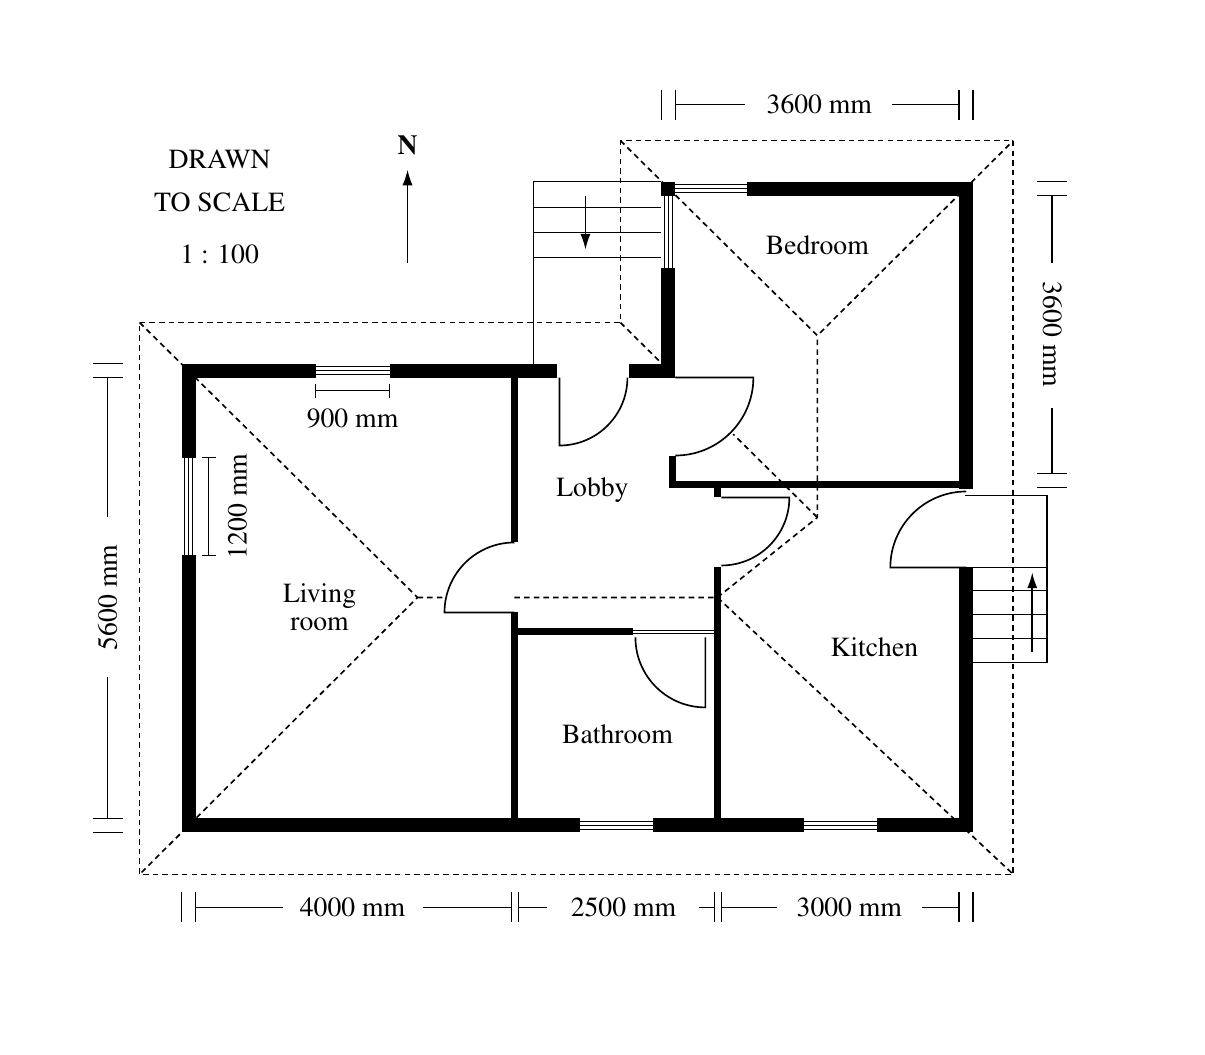
\begin{tikzpicture}[x=0.0127cm,y=-0.0127cm]
% dashed roof outline and hips
\begin{scope}[even odd rule]
% door swings knocked out of the dashed lines (checker: no slash through the doors)
\clip (-50,-50) rectangle (1100,950)
  (482,300) -- (553,300) arc[start angle=0,end angle=90,radius=71] -- cycle
  (598,300) -- (679,300) arc[start angle=0,end angle=90,radius=81] -- cycle
  (644,420) -- (715,420) arc[start angle=0,end angle=90,radius=71] -- cycle
  (437,535) -- (364,535) arc[start angle=180,end angle=270,radius=73] -- cycle
  (628,560) -- (628,633) arc[start angle=90,end angle=180,radius=73] -- cycle
  (889,490) -- (810,490) arc[start angle=180,end angle=270,radius=79] -- cycle;
\draw[aux] (62,245) -- (543,245) -- (543,63) -- (936,63) -- (936,797) -- (62,797) -- cycle;
\draw[aux] (62,245) -- (340,520) -- (62,797);
\draw[aux] (340,520) -- (640,520) -- (936,797);
\draw[aux] (640,520) -- (740,440) -- (740,258);
\draw[aux] (543,63) -- (740,258) -- (936,63);
\draw[aux] (543,245) -- (740,440);
\end{scope}
% stairs top
\draw (456,286) -- (456,104) -- (584,104);
\foreach \y in {130,155,180} \draw (456,\y) -- (584,\y);
\draw[->] (508,118) -- (508,172);
% stairs right
\draw (888,418) -- (970,418) -- (970,585) -- (896,585);
\foreach \y in {490,513,537,561} \draw (896,\y) -- (970,\y);
\draw[->] (955,575) -- (955,495);
% thick external walls
\fill (104,286) rectangle (238,300);
\fill (312,286) rectangle (480,300);
\fill (552,286) rectangle (598,300);
\fill (104,286) rectangle (118,380);
\fill (104,478) rectangle (118,755);
\fill (104,741) rectangle (503,755);
\fill (576,741) rectangle (727,755);
\fill (800,741) rectangle (896,755);
\fill (882,490) rectangle (896,755);
\fill (882,104) rectangle (896,412);
\fill (670,104) rectangle (896,118);
\fill (584,104) rectangle (598,118);
\fill (584,190) rectangle (598,300);
% interior walls
\fill (434,300) rectangle (441,465);
\fill (434,535) rectangle (441,741);
\fill (441,551) rectangle (556,558);
\fill (637,404) rectangle (644,420);
\fill (637,490) rectangle (644,741);
\fill (592,404) rectangle (882,411);
\fill (592,378) rectangle (599,411);
% windows (thin double lines)
\draw[line width=0.4pt] (238,289) -- (312,289) (238,297) -- (312,297) (238,293) -- (312,293);
\draw[line width=0.4pt] (107,380) -- (107,478) (115,380) -- (115,478) (111,380) -- (111,478);
\draw[line width=0.4pt] (503,744) -- (576,744) (503,752) -- (576,752) (503,748) -- (576,748);
\draw[line width=0.4pt] (727,744) -- (800,744) (727,752) -- (800,752) (727,748) -- (800,748);
\draw[line width=0.4pt] (598,107) -- (670,107) (598,115) -- (670,115) (598,111) -- (670,111);
\draw[line width=0.4pt] (587,118) -- (587,190) (595,118) -- (595,190) (591,118) -- (591,190);
\draw[line width=0.4pt] (556,553) -- (637,553) (556,556) -- (637,556);
% doors (angles: 0 right, 90 down, 180 left, 270 up on the page)
\draw (482,300) -- (482,368) arc[start angle=90,end angle=0,radius=68];
\draw (598,300) -- (676,300) arc[start angle=0,end angle=90,radius=78];
\draw (644,420) -- (712,420) arc[start angle=0,end angle=90,radius=68];
\draw (437,535) -- (367,535) arc[start angle=180,end angle=270,radius=70];
\draw (628,560) -- (628,630) arc[start angle=90,end angle=180,radius=70];
\draw (889,490) -- (813,490) arc[start angle=180,end angle=270,radius=76];
% room labels
\node at (740,168) {Bedroom};
\node at (515,413) {Lobby};
\node[align=center] at (242,530) {Living\\[-2pt]room};
\node at (797,570) {Kitchen};
\node at (540,657) {Bathroom};
\node at (142,82) {DRAWN};
\node at (142,125) {TO SCALE};
\node at (142,177) {1 : 100};
% north arrow
\draw[->] (330,185) -- (330,92);
\node[font=\bfseries] at (330,68) {N};
% window dimensions
\draw (238,313) -- (312,313); \draw (238,306) -- (238,320) (312,306) -- (312,320);
\node at (275,341) {900 mm};
\draw (131,380) -- (131,478); \draw (124,380) -- (138,380) (124,478) -- (138,478);
\node[rotate=90] at (160,429) {1200 mm};
% bottom dimension line
\foreach \x in {104,118,434,441,637,644,882,896} \draw (\x,815) -- (\x,845);
\draw (118,830) -- (205,830) (345,830) -- (434,830);
\draw (441,830) -- (470,830) (622,830) -- (637,830);
\draw (644,830) -- (700,830) (845,830) -- (882,830);
\node at (275,830) {4000 mm};
\node at (546,830) {2500 mm};
\node at (772,830) {3000 mm};
% top dimension
\foreach \x in {584,598,882,896} \draw (\x,12) -- (\x,42);
\draw (598,27) -- (668,27) (815,27) -- (882,27);
\node at (742,27) {3600 mm};
% right dimension
\foreach \y in {104,118,396,410} \draw (960,\y) -- (990,\y);
\draw (975,118) -- (975,185) (975,330) -- (975,396);
\node[rotate=-90] at (975,257) {3600 mm};
% left dimension
\foreach \y in {286,300,741,755} \draw (15,\y) -- (45,\y);
\draw (30,300) -- (30,440) (30,600) -- (30,741);
\node[rotate=90] at (30,520) {5600 mm};
\end{tikzpicture}
\end{document}